% Foliensatz: "AFu-Kurs nach DJ4UF" von DK0TU, Amateurfunkgruppe der TU Berlin
% Lizenz: CC BY-NC-SA 3.0 de (http://creativecommons.org/licenses/by-nc-sa/3.0/de/)
% Autoren: Martin Deutschmann DM7MD <martin.deutschmann@campus.tu-berlin.de>

\documentclass[aspectratio=169]{beamer}

\usepackage[ngerman]{babel} % deutsche Worttrennung etc.
\usepackage[utf8]{inputenc} % UTF8 Text

\usepackage[super, comma, numbers, square, sort]{natbib}

\usepackage{hyperref}       % Hyperref Package für bessere Referenzen (todo)
\hypersetup{
	colorlinks=false,       %   false: boxed links; true: colored links
    %linkcolor=white,       %   color of internal links (change box color with linkbordercolor)
    citecolor=red,          %   color of links to bibliography
    filecolor=white,        %   color of file links
    urlcolor=blue           %   color of external links
}

\usepackage{multirow}
\usepackage{wasysym}  % Math Symbols like \permil
%\usepackage{colortbl}
%\usepackage{subscript}
%\usepackage{caption}
%\usepackage{setspace}
%\usepackage{xcolor}        % benutze CodeListe

% Footnote
%\usepackage{hanging}
%
%\setbeamertemplate{footnote}{%
%  \hangpara{2em}{1}%
%  \makebox[2em][l]{\insertfootnotemark}\footnotesize\insertfootnotetext\par%
%}


%\usepackage{pgf}
%\usepackage{tikz}
%\usetikzlibrary{arrows,automata}
%\usetikzlibrary{positioning}
%
%\tikzset{
%    state/.style={
%           rectangle,
%           rounded corners,
%           draw=black, very thick,
%           minimum height=2em,
%           minimum width=2pt,
%           inner sep=2pt,
%           text centered,
%           },
%}

%\usepackage{listings}
%\lstset{basicstyle=\small, numberstyle=\tiny, extendedchars=true, numbers=left, numbersep=5pt}
%\lstset{showtabs=false, showspaces=false, showstringspaces=false}
%%\lstset{backgroundcolor=\color{white!75!lightgray}, , frame=single}
%%\lstset{backgroundcolor=\color{white}}
%%\lstset{backgroundcolor=none}
%\lstset{keywordstyle=\color{blue!50!gray},  identifierstyle=\color{black}}
%\lstset{commentstyle=\color{green!50!gray}, stringstyle=\color{red!50!gray}}
%\lstset{language=C, fontadjust=true, tabsize=2, breaklines=true}
%\lstset{backgroundcolor=\color{white!75!lightgray}, caption=\lstname, frame=single}
%\lstset{emphstyle=\color{black}\fbox}
%
%% Keine "Listing:"-Caption
%\captionsetup{labelformat=empty,labelsep=none}
%
%% für mathematische Umgebungen
%\usepackage{amsmath,amsfonts,amssymb}
%
%\lstdefinestyle{Bash}{
%language=Bash,
%frame=single,
%rulecolor=\color{black},
%backgroundcolor=\color{gray!50},
%keywordstyle=\color{black},
%identifierstyle=,
%commentstyle=\color{black},
%stringstyle=\color{magenta!65!white},
%showstringspaces=false,
%basicstyle=\footnotesize\ttfamily\color{black},
%numbers=none,
%breaklines=true,
%captionpos=b
%}

%\usepackage{listings}
%
%\lstdefinestyle{basic}{
%    captionpos=t,%
%    basicstyle=\footnotesize\ttfamily,%
%    numberstyle=\tiny,%
%    numbers=left,%
%    stepnumber=1,%
%    frame=single,%
%    showspaces=false,%
%    showstringspaces=false,%
%    showtabs=false,%
%    %
%    keywordstyle=\color{blue},%
%    identifierstyle=,%
%    commentstyle=\color{gray},%
%    stringstyle=\color{magenta}%
%}



% fließende Boxen haben keinen Abstand
%\fboxsep0mm

% inkludiere Creative Commons Helper
%%%%%%%%%%%%%%%%%%%%%%%%%%%%%%%%%%%%%%%%%%%%%%%%%%%%%%%%%%%%%%%%
%% ccBeamer 0.1, 2007-07-02                                   %%
%% Written by Sebastian Pipping <webmaster@hartwork.org>      %%
%% ---------------------------------------------------------- %%
%% Licensed under Creative Commons Attribution-ShareAlike 3.0 %%
%% http://creativecommons.org/licenses/by-sa/3.0/             %%
%%%%%%%%%%%%%%%%%%%%%%%%%%%%%%%%%%%%%%%%%%%%%%%%%%%%%%%%%%%%%%%%


%% Images
\newcommand{\CcImageBy}[1]{%
	
\includegraphics[scale=#1]{texdata/creative_commons/cc_by_30.pdf}%
}
\newcommand{\CcImageCc}[1]{%
	
\includegraphics[scale=#1]{texdata/creative_commons/cc_cc_30.pdf}%
}
\newcommand{\CcImageDevNations}[1]{%
	
\includegraphics[scale=#1]{texdata/creative_commons/cc_dev_nations_30.pdf}%
}
\newcommand{\CcImageNc}[1]{%
	
\includegraphics[scale=#1]{texdata/creative_commons/cc_nc_30.pdf}%
}
\newcommand{\CcImageNd}[1]{%
	
\includegraphics[scale=#1]{texdata/creative_commons/cc_nd_30.pdf}%
}
\newcommand{\CcImagePd}[1]{%
	
\includegraphics[scale=#1]{texdata/creative_commons/cc_pd_30.pdf}%
}
\newcommand{\CcImageSa}[1]{%
	
\includegraphics[scale=#1]{texdata/creative_commons/cc_sa_30.pdf}%
}
\newcommand{\CcImageSampling}[1]{%
	
\includegraphics[scale=#1]{texdata/creative_commons/cc_sampling_30.pdf}%
}
\newcommand{\CcImageSamplingPlus}[1]{%
	
\includegraphics[scale=#1]{texdata/creative_commons/cc_sampling_plus_30.pdf}%
}


%% Groups
\newcommand{\CcGroupBy}[2]{% zoom, gap
	\CcImageCc{#1}\hspace*{#2}\CcImageBy{#1}%
}
\newcommand{\CcGroupByNc}[2]{% zoom, gap
	\CcImageCc{#1}\hspace*{#2}\CcImageBy{#1}\hspace*{#2}\CcImageNc{#1}%
}
\newcommand{\CcGroupByNcNd}[2]{% zoom, gap
	\CcImageCc{#1}\hspace*{#2}\CcImageBy{#1}\hspace*{#2}\CcImageNc{#1}\hspace*{#2}\CcImageNd{#1}%
}
\newcommand{\CcGroupByNcSa}[2]{% zoom, gap
	\CcImageCc{#1}\hspace*{#2}\CcImageBy{#1}\hspace*{#2}\CcImageNc{#1}\hspace*{#2}\CcImageSa{#1}%
}
\newcommand{\CcGroupByNd}[2]{% zoom, gap
	\CcImageCc{#1}\hspace*{#2}\CcImageBy{#1}\hspace*{#2}\CcImageNd{#1}%
}
\newcommand{\CcGroupBySa}[2]{% zoom, gap
	\CcImageCc{#1}\hspace*{#2}\CcImageBy{#1}\hspace*{#2}\CcImageSa{#1}%
}
\newcommand{\CcGroupDevNations}[2]{% zoom, gap
	\CcImageCc{#1}\hspace*{#2}\CcImageDevNations{#1}%
}
\newcommand{\CcGroupNcSampling}[2]{% zoom, gap
	\CcImageCc{#1}\hspace*{#2}\CcImageNc{#1}\hspace*{#2}\CcImageSampling{#1}%
}
\newcommand{\CcGroupPd}[1]{% zoom
	\CcImagePd{#1}%
}
\newcommand{\CcGroupSampling}[1]{% zoom
	\CcImageSampling{#1}%
}
\newcommand{\CcGroupSamplingPlus}[1]{% zoom
	\CcImageSamplingPlus{#1}%
}


%% Text
\newcommand{\CcLongnameBy}{Attribution}
\newcommand{\CcLongnameByNc}{Attribution-NonCommercial}
\newcommand{\CcLongnameByNcNd}{Attribution-NoDerivs}
\newcommand{\CcLongnameByNcSa}{Attribution-NonCommercial-ShareAlike}
\newcommand{\CcLongnameByNd}{Attribution-NoDerivs}
\newcommand{\CcLongnameBySa}{Attribution-ShareAlike}

\newcommand{\CcNote}[1]{% longname
	This work is licensed under the \textit{Creative Commons #1 3.0 License}.%
}


% generelles Thema auswählen
\usetheme{Goettingen} %Berlin spart ohne Sidebar allerdings angenehm Platz
% AnnArbor | Antibes | Bergen | Berkeley | Berlin | Boadilla | boxes | CambridgeUS | Copenhagen | Darmstadt | default | Dresden | Frankfurt | Goettingen | Hannover | Ilmenau | JuanLesPins | Luebeck | Madrid | Malmoe | Marburg | Montpellier | PaloAlto | Pittsburgh | Rochester | Singapore | Szeged | Warsaw

% Farben wählen
\usecolortheme{beetle}
% beaver | beetle | crane | default | dolphin | dove | fly | lily | orchid | rose | seagull | seahorse | sidebartab | structure | whale | wolverine

% Setze alle Farben auf Grau und Weiß
%\definecolor{craneorange}{RGB}{64,64,64}
%\definecolor{craneblue}{RGB}{255,255,255}

% Schriftart wählen
\usefonttheme{default}
% default | professionalfonts | serif | structurebold | structureitalicserif | structuresmallcapsserif

% Innere Themen(Kopf-, Fuß-, Sidebar usw)
%\useinnertheme{default}
\useinnertheme{circles}
% default | inmargin | rectangles | rounded | circles

% Äußere Themen (Anordnung der inneren, grenzen der Folien etc.)
\useoutertheme{infolines}
% default | infolines | miniframes | shadow | sidebar | smoothbars | smoothtree | split | tree

% Deaktiviere Navigations-Symbole ({} -> leer)
\setbeamertemplate{navigation symbols}{}
%\setbeamertemplate{navigation symbols}{\large \ifnum \insertframenumber <10 0\fi\insertframenumber/\inserttotalframenumber\vspace*{0.2ex}}

% Zeige ein Hintergrundbild
\setbeamertemplate{background canvas}{
        \hspace*{-2.0cm}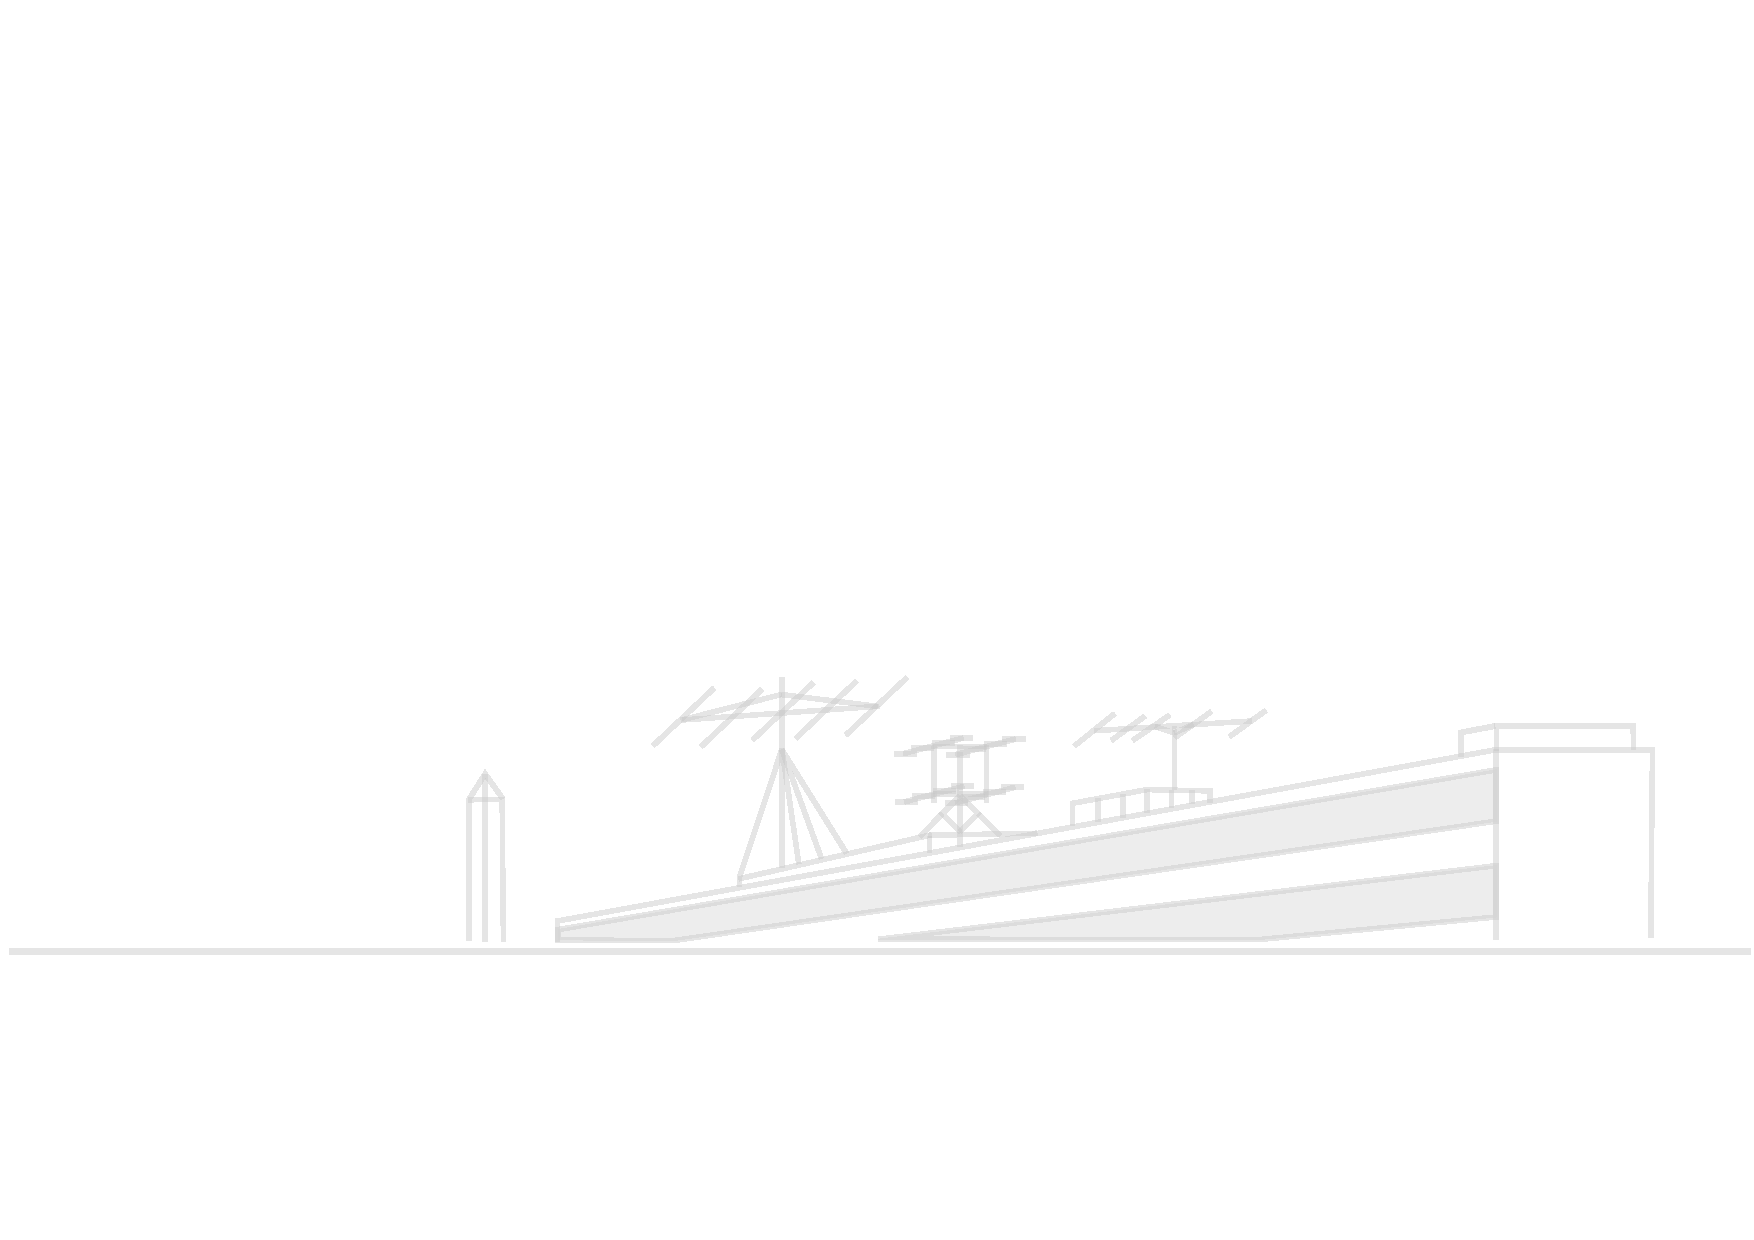
\includegraphics[width=17.8cm]{texdata/dk0tu_rooftop_background.pdf}
}

% Foliennummer einfügen
\setbeamertemplate{footline}[frame number]
%\setbeamertemplate{footline}{}

% Ändere das Zeichen vor jedem item
%\setbeamertemplate{itemize item}{\color{craneorange}$\blacktriangleright$}
%\setbeamertemplate{itemize subitem}{\color{craneorange}$\triangleright$}
%\setbeamertemplate{itemize subsubitem}{\color{craneorange}$\blacktriangleright$}

% Ändert die Blöcke 
\setbeamertemplate{blocks}[rounded][shadow=true]
% default | rounded [shadow=true|false]

%
% Eigene Kommandos
%

% Hack to get natbib and beamer working together. "The beamer user guide suggests
% that only the manual bibliography entry approach is supported"
% on some system it works out of the box, sometimes you need the hack :-(
% so check it --dl7bst
\ifdefined\newblock
    \relax
\else
    \newcommand{\newblock}{}
\fi

% \includedia command to generate png out of a dia file
% NEEDS installed dia and pdflatex option --shell-escape
\newcommand{\includedia}[1]{
    \immediate\write18{/usr/bin/dia #1.dia -e #1_diatmp.png -t png}
}

% RICHIG GROSSER FONT!
\newfont{\bigfont}{cmr10 at 144pt}
\newfont{\smallfont}{cmr10 at 8pt}

% Römische Ziffern
\makeatletter
\newcommand{\rmnum}[1]{\romannumeral #1}
\newcommand{\Rmnum}[1]{\expandafter\@slowromancap\romannumeral #1@}
\makeatother

% Schwarze Überschrift
%\setbeamercolor{frametitle}{fg=black}
%\setbeamercolor{title}{fg=black}

% Item- und Box-Farben
\definecolor{deepBlue}{HTML}{000066}
\setbeamercolor{itemize item}{fg=deepBlue}
\setbeamercolor{itemize subitem}{fg=deepBlue}
\setbeamercolor{description item}{fg=deepBlue}
\setbeamercolor{block title}{fg=deepBlue!100, bg=blue!15}
\setbeamercolor{block body}{fg=black, bg=blue!5}
\setbeamercolor{block title alerted}{fg=deepBlue, bg=red!75}
\setbeamercolor{block body alerted}{fg=black, bg=red!15}
\setbeamercolor*{block title example}{fg=blue!50, bg=blue!10}
\setbeamercolor*{block body example}{fg= blue, bg=blue!5}

%\setbeamercolor{section in head/foot}{parent=palette primary}
%\setbeamercolor{subsection in head/foot}{parent=palette secondary}
%\setbeamercolor{sidebar}{fg=darkblue,bg=yellow!90!orange}
%\setbeamercolor{title in sidebar}{fg=darkblue}
%\setbeamercolor{author in sidebar}{fg=darkblue}
%\setbeamercolor{section in sidebar}{fg=darkblue!10!black}
%\setbeamercolor{subsection in sidebar}{fg=darkblue!50!black}

% Titlepage Infos
\title{AFu-Kurs nach DJ4UF}
\author[DKØTU]{DKØTU\\ \footnotesize{Amateurfunkgruppe der TU Berlin}}
\institute[DKØTU]{\url{http://www.dk0tu.de} }

% PDF-Eigenschaften
\subject{DK0TU-Amateurfunkkurs nach DJ4UF}
\keywords{Amateurfunk Kurs HAM Radio Course CC-BY-NC-SA OpenSource TU Berlin DK0TU}

\subtitle{Technik A17: \\
           Schaltungstechnik \\[2em]}
\date{Stand 22.06.2015}
 \begin{document}

\begin{frame}
    \titlepage
    \vfill
    \begin{center}
        \ccbyncsaeu\\
        {\tiny This work is licensed under the \em{Creative Commons Attribution-NonCommercial-ShareAlike 3.0 License}.}\\[0.5ex]
         \tiny Amateurfunkgruppe der Technische Universität Berlin (AfuTUB), DKØTU
         %\includegraphics[scale=0.5]{img/DK0TU_Logo.pdf}
    \end{center}
\end{frame}


\section*{Röhren PA mit Pi-Filter}
\begin{frame}
    \frametitle{HF-Verstärker mit Röhren}
    \begin{center}
        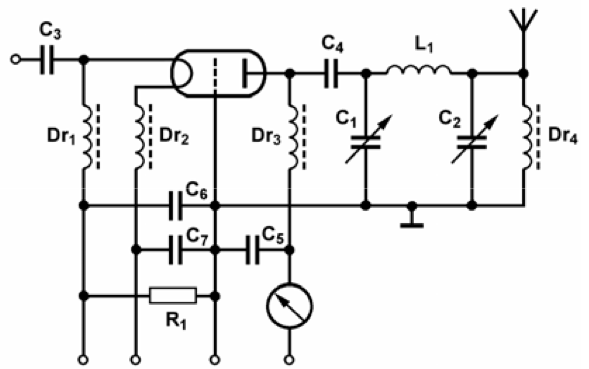
\includegraphics[width=0.6\textwidth]{a17/TG313.png}\\
        \tiny TG313 \hyperlink{refs}{\cite{bna}}
     	\begin{enumerate} \Large
			\item Röhrenendstufe mit Pi-Filter am Ausgang
    	\end{enumerate}
    \end{center}
\end{frame}

\begin{frame}
\frametitle{Wissenswertes zu Röhren PAs mit Pi-Filtern}
\begin{center}
\begin{itemize}
	\item	Haben höheren Wirkungsgrad als Transistorendstufen
	\item	Da mit hohen Spannungen und geringen Strömen gearbeitet wird
	\item	Die meisten Verluste treten durch Ströme in den Spulen auf
	\item	Benötigt zur Arbeitspunkteinstellung am Gitter eine geringere Spannung als an der Katode
	\item	Dafür kann eine Konstantspannungsquelle, oder ein Widerstand genutzt werden
	\item	Pi-Filter dient der Impedanzanpassung
\end{itemize}
\end{center}
\end{frame}

\begin{frame}
\frametitle{Das Abstimmen einer Röhren PAs mit Pi-Filtern}
\begin{center}
\begin{itemize}
	\item	$C_1$ ist für die Resonanz des Kreises verantwortlich
	\item	Wird auch Abstimmkondensator, Plate oder Tune bezeichnet
	\item	$C_2$ dient der Einstellung der Lastimpedanz (LOAD)
	\item	Zuerst stellt man $C_1$ und $C_2$ auf max
	\item	$C_1$ auf Dip im Anodenstrom stellen (Resonanz)
	\item	Nun mit $C_2$ einen etwas höheren Anodenstrom einstellen (Leistung auskoppeln)
	\item	Vorgang mit $C_1$ und $C_2$ wechselseitig wiederholen bis maximale Ausgangsleistung erreicht ist
	\item	Nach dem Abstimmvorgang sollte noch ein Dip von ca. 10\% verbleiben 
\end{itemize}
\end{center}
\end{frame}

\begin{frame}
    \begin{center} \Large
        \begin{block}{TG310}
		\large  LC-Schaltungen unmittelbar vor und hinter einem HF-Leistungsverstärker dienen\\
    	\end{block}
        \begin{tabular}{|c|c|}
        \hline
        A & zur Verringerung der rücklaufenden \\ 	
        " " & Leistung bei Fehlanpassung. \\ \hline
        B & zur optimalen Einstellung des \\ 
        " " & Arbeitspunktes nach Betrag und Phase. \\ \hline
        C & zur optimalen Anpassung der \\
        " " & Ein- und Ausgangsimpedanzen.\\ \hline
        D & zur Erhöhung des HF-Wirkungsgrades \\
        " " & der Verstärkerstufe.\\ \hline
        \end{tabular}
    \end{center}
\end{frame}
\begin{frame}
    \begin{center} \Large
        \begin{block}{TG310}
		\large  LC-Schaltungen unmittelbar vor und hinter einem HF-Leistungsverstärker dienen\\
    	\end{block}
        \begin{tabular}{|c|c|}
        \hline
        A & zur Verringerung der rücklaufenden \\ 	
        " " & Leistung bei Fehlanpassung. \\ \hline
        B & zur optimalen Einstellung des \\ 
        " " & Arbeitspunktes nach Betrag und Phase. \\ \hline
        C & zur optimalen Anpassung der \\
        X & Ein- und Ausgangsimpedanzen.\\ \hline
        D & zur Erhöhung des HF-Wirkungsgrades \\
        " " & der Verstärkerstufe.\\ \hline
        \end{tabular}
    \end{center}
\end{frame}

\section*{2m-FM Endstufe}
\begin{frame}
    \begin{center}
        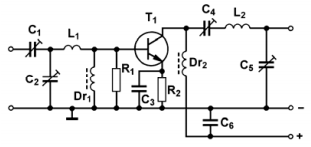
\includegraphics[width=1\textwidth]{a17/TG311.png}\\
       $2m$-FM Endstufe{bna}
    \end{center}
\end{frame}
\begin{frame}
\frametitle{Wichtiges hier zu}
\begin{itemize}
	\item	Zur Abgleich des Verstärkers wird eine $50 \Omega$ Dummy-Load für UKW angeschlossen
	\item	Dann wird die Eingangsleistung erhöht, bis der Strom etwas ansteigt
	\item	Nun abwechselnd die Ausgangskondensatoren verstellen bis die Leistung etwa konstant bleibt
	\item	Danach wird der Vorgang mit den Eingangskondensatoren wiederholt
	\item	Dann wird die Eingangsleistung erhöht bis die Schaltung einen Strom von etwa $2,7 A$ aufnimmt (= Nennstrom der Schaltung)
	\item	Anschließend wird der alles bei wiederholt
	\item	Um Eigenschwingungen zu vermindern kann man die Eingangsimpedanz des Transistors  mit einem Widerstand dämpfen
	\item	Oder den Emitteranschluss mit einer Ferritperle versehen.
\end{itemize}
\end{frame}

\begin{frame}
\frametitle{Und noch ein paar Infos}
\begin{itemize}
	\item	Diese Schaltung sollte in ein Metallgehäuse montiert werden
	\item	Am Besten noch mit Trennwand hinter dem Transistor
	\item	Der Verstärker arbeitet im C-Betrieb
	\item	Und kann nur CW und FM
	\item	er kann \textbf{kein SSB} 
\end{itemize}
\end{frame}

\section*{Linearverstärker}
\begin{frame}
    \begin{center}
        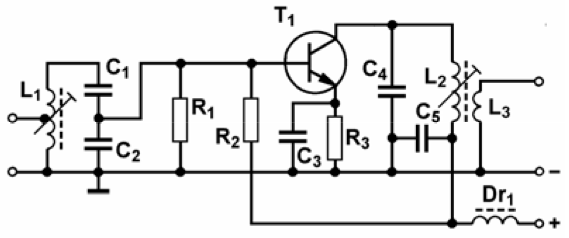
\includegraphics[width=1\textwidth]{a17/TG222.png}\\
       Linearverstärker\cite{bna}
    \end{center}
\end{frame}

\begin{frame}
\frametitle{Good to know}
\begin{itemize}
	\item	HF-Verstärker sollen möglichst verzerrungsfrei(linear) verstärken
	\item	Einen solchen Verstärker kann man mit zwei Transistoren im Gegentakt-B-Betrieb aufbauen
	\item	Oder mit einem Transistor im AB-Betrieb
	\item	Bei kleinen Signalen arbeitet der Transistor dann im A-Betrieb und bei größeren im B-Betrieb
	\item	$R_1$ und $R_2$ bestimmen den Arbeitspunkt des Transistors
	\item	Der Schwingkreis $L_1 - C_1 - C_2$ schafft eine doppelte Resonanztransformation
	\item	Das Verhältnis von $C_1$ zu $C_2$ bestimmt die Anpassung an die Basis des Transistors
	\item	Die Mittelanzapfung an $L_1$ erzeugt den üblichen $50 \Omega$ Eingangswiderstand
	\item	Der Ausgang wird normal transformiert über $L_2$ zu $L_3$
\end{itemize}
\end{frame}

\section*{Detektor-Empfänger}
\begin{frame}
\frametitle{Der Detektorempfänger}
    \begin{center}
        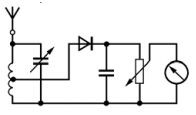
\includegraphics[width=0.8\textwidth]{a17/TJ601.png}\\
       Detektorempfänger \cite{bna}
    \end{center}
\end{frame}

\section*{Aufbau von Oszillatoren}
\begin{frame}
\frametitle{Aufbau von Oszillatoren: Let's swing :)}
\begin{itemize}
	\item	Ls und Cs sind temperaturabhängig
	\item	Spulen dehnen sich aus, dadurch steigt ihr Querschnitt und die Induktivität
	\item	Deshalb nutzt man dafür Kondensatoren mit negativen Temperaturkoeffizienten
	\item	wie z.B. Styroflexkondensatoren
	\item	Dies alles beeinflusst die Frequenz
	\item	Also Oszis weg von Wärmequellen ;)
	\item	extra stabilisierte Spannungsversorgung verhindert ein verzerren der Frequenz durch den Transistor
	\item	Und immer gut schirmen
    \item   Absorptionsfrequenzmesser
\end{itemize}
\end{frame}

\section*{Die Dummyload}

\begin{frame}
\frametitle{Die Dummie-Load}
\begin{itemize}
	\item	Im Prinzip ist die Dummy-Load ein Widerstand der für hohe Frequenzen und Leistungen gebaut wurde
	\item	Dabei soll sie wenig kapazitive und noch wichtiger, wenig induktive Anteile haben
	\item	Gut eignen sich Schichtwiderstände 
\end{itemize}
\end{frame}

\section*{Netzteil und Stabilisierung}
\begin{frame}
    \begin{center}
        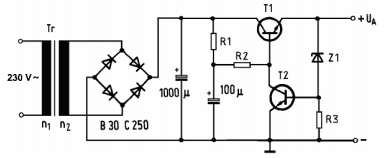
\includegraphics[width=1\textwidth]{a17/TD306.png}\\
       Netzteil \cite{bna}
    \end{center}
\end{frame}

\begin{frame}
\frametitle{Wie funzt das jetzt?}
\begin{itemize}
	\item	Fixe Ausgangspannung, Z-Spannung + $0,6V$ $U_{BE}$ für $T_2$
	\item	$U_a$ sinkt $\rightarrow$	$I_{B,T2}$ sinkt $\rightarrow$ $U_{R_1,R_2}$ sinkt $\rightarrow$ $U_B$ steigt $\rightarrow$ $T_2$ leitet besser $\rightarrow$ $U_a$ steigt
\end{itemize}
\end{frame}

\subsection*{Festpannungsregler}
\begin{frame}
    \begin{center}
        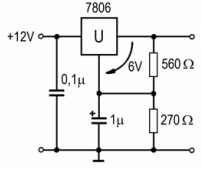
\includegraphics[width=0.6\textwidth]{a17/TD319.png}\\
       Festpannungsregler \cite{bna}
    \end{center}
\end{frame}

\begin{frame}
\frametitle{Lass uns das regeln wie echte Regler}
\begin{itemize}
	\item	Viel freundlicher im Umgang als z.B. die Z-Diodenschaltung
	\item	Benötigen nur noch Kondensatoren drum herum
	\item	brauchen etwa $15 \%$ mehr Spannung als sie stabilisieren sollen
	\item	Sollte der Regler mal zu wenig Strom liefern, kann er mit einem Transistor erweitert werden
\end{itemize}
\end{frame}

\begin{frame}
    \begin{center} \Large
        \begin{block}{TD319}
		\large Welche Ausgangsspannung entsteht mit folgender Spannungsregler-Schaltung?\\
		\begin{center}
		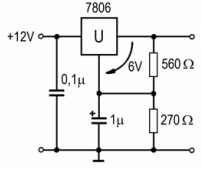
\includegraphics[width=0.3\textwidth]{a17/TD319.png}\\
		\end{center}
    	\end{block}
        \begin{tabular}{|c|c|}
        \hline
        A & 6V \\ \hline
        B & 8,9V \\ \hline
        C & 18V \\ \hline
        D & 14,9V \\ \hline
        \end{tabular}
    \end{center}
\end{frame}
\begin{frame}
    \begin{center} \Large
        \begin{block}{TD319}
		\large Welche Ausgangsspannung entsteht mit folgender Spannungsregler-Schaltung?\\
		\begin{center}
		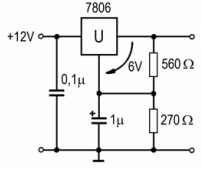
\includegraphics[width=0.3\textwidth]{a17/TD319.png}\\
		\end{center}
    	\end{block}
        \begin{tabular}{|c|c|}
        \hline
        A & 6V \\ \hline
        X & 8,9V \\ \hline
        C & 18V \\ \hline
        D & 14,9V \\ \hline
        \end{tabular}
    \end{center}
\end{frame}

\begin{frame}
    \begin{center} \Large
        \begin{block}{TD312}
		\large Die Ausgangsspannung zwischen A und B in der Schaltung beträgt ungefähr?\\
		\begin{center}
		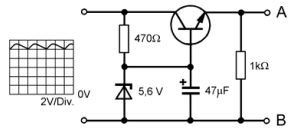
\includegraphics[width=0.5\textwidth]{a17/TD312.png}\\
		\end{center}
    	\end{block}
        \begin{tabular}{|c|c|}
        \hline
        A & 5,6V \\ \hline
        B & 11,2V \\ \hline
        C & 6,2V \\ \hline
        D & 5V \\ \hline
        \end{tabular}
    \end{center}
\end{frame}
\begin{frame}
    \begin{center} \Large
        \begin{block}{TD312}
		\large Die Ausgangsspannung zwischen A und B in der Schaltung beträgt ungefähr?\\
		\begin{center}
		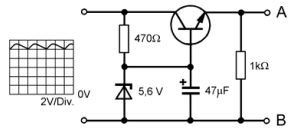
\includegraphics[width=0.5\textwidth]{a17/TD312.png}\\
		\end{center}
    	\end{block}
        \begin{tabular}{|c|c|}
        \hline
        A & 5,6V \\ \hline
        B & 11,2V \\ \hline
        C & 6,2V \\ \hline
        X & 5V \\ \hline
        \end{tabular}
    \end{center}
\end{frame}

\subsection*{Schaltnetzteil}
\begin{frame}
    \begin{center}
        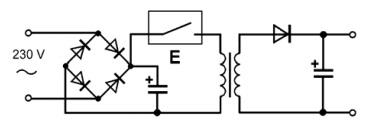
\includegraphics[width=1\textwidth]{a17/TD317.png}\\
       Schaltnetzteil \cite{bna}
    \end{center}
\end{frame}

\begin{frame}
\frametitle{So einfach gehts}
\begin{itemize}
	\item	Will man den Trafo in einem Netzteil verkleinern, brauch man höhere Spannungen
	\item	Lösung des Problems, man richtet die Wechselspannung gleich, zerhackstückelt diese dann per elektronischen Schalter, transformiert sie dann und richtet sie wieder gleich
	\item	Schaltfrequenzen gehen bis in den MHz-Bereich
	\item	Erzeugt dafür aber Oberwellen die auf KW stören können
\end{itemize}
\end{frame}

\section*{Mechanik \& Sicherheit}
\begin{frame}
\frametitle{Was für die Bastler}
\begin{itemize}
	\item	Ich kann es nicht oft genug sagen: "Immer an die Abschirmung denken"
	\item	Am Besten Metallgehäuse nutzten
	\item	Braucht das Gerät Netzspannung, muss das gesamte Gehäuse geerdet werden
	\item	Bei HF-Verstärkern in der Versorgung auch noch die HF rausfiltern
\end{itemize}
\end{frame}

\renewcommand{\refname}{Referenzen}

\hypertarget{refs}{}
\textcolor{white}{} \\ %\vspace{} geht nicht
\Large Referenzen/Links
\footnotesize

\begin{thebibliography}{}
    \bibitem{darc}  DARC Online-Lehrgang Lektion A17:
                    \url{http://www.darc.de/referate/ajw/ausbildung/darc-online-lehrgang/technik-klasse-a/technik-a17/}
    \bibitem{wm} 	Wikimedia:
	\bibitem{bna}   Fragenkatalog Bundesnetzargentur Technik Klasse A:                   
                    \url{https://www.bundesnetzagentur.de/SharedDocs/Downloads/DE/Sachgebiete/Telekommunikation/Unternehmen_Institutionen/Frequenzen/Amateurfunk/Fragenkatalog/TechnikFragenkatalogKlasseAf252rId9014pdf.pdf?__blob=publicationFile&v=3}
    \bibitem{fi}    Freie Inhalte (DK0TU):
                    \url{http://www.dk0tu.de/Projekte/Freie_Inhalte/}
\end{thebibliography} 

% Hier könnte noch eine Kontaktfolie stehen

\end{document}

